\chapter[Ferramentas de Gerência de Requisitos]{Ferramentas de Gerência de Requisitos}

Ferramentas de gerência de requisitos foram feitas com o intuito de auxiliar os responsáveis pelo desenvolvimento do software a gerir os requisitos. Em geral, essas ferramentas armazenam, coletam, aplicam mudanças, inserem, atualizam e excluem, mantém versões dos requisitos. Apesar disso, as ferramentas possuem divergências entre suas funcionalidades, assim, cada programa atende a realidade de uma empresa \cite{ananias2009}.

\section{Analise das ferramentas}

\subsection{OSRMT}
O Open Source Requirements Management Tool (OSRMT) é uma ferramenta livre com licença General Public License (GPL) desenvolvida em Java. A ferramenta disponibiliza a possibilidade de se fazer o rastreamento total dos requisitos, tendo também, gerência dos requisitos bem como dos componentes de produtos de trabalho \cite{ananias2009}.

O software em questão tem portabilidade ao Windows, Linux e Mac e possibilita dois modos distintos, servidor e cliente. No modo servidor, o software pode ser utilizado via web, facilitando o contado com os stakeholders, utilizando o Tomcat ou JBoss para prover o acesso. No modo cliente, o software tem que ser instalado em um desktop e configurado com um banco de dados, possibilitando a vantagem de funcionar de modo offline.

A ferramenta oferece:
\begin{itemize}
    \item Cadastro de autor, origem e motivo da necessidade de cada requisito;
    \item Cadastro de casos de uso do requisito, ajudando a prover e avaliar o impacto do requisito no projeto do software;
    \item Cadastro do status do requisito;
    \item Cadastro de origem dos requisitos, possibilitando a atribuição de categorias nos requisitos, de modo a auxiliar na derivação dos mesmos;
\end{itemize}
               
As duas principais tarefas de uma ferramenta de gerenciamento de requisitos de software são: gerenciar mudanças nos requisitos acordados e gerenciar os relacionamentos entre os requisitos \cite{dourado2008} sendo que essas funcionalidades são contempladas pela OSRMT, possibilitando um bom rastreamento e facilitando possíveis mudanças.

Outras funcionalidades:
\begin{itemize}
    \item Definição de artefatos e entrada de dados (características, requisitos, código fonte, casos de teste);
    \item Organização hierárquica e controle de versão dos artefatos;
    \item Rastreabilidade, gráficos identificando todas as dependências entre os artefatos selecionados para determinar o impacto de mudanças;
    \item Relatórios padronizados, geração de relatórios em \textit{Portable Document Format} (PDF) e \textit{Hyper Text Markup Language} (HTML);
    \item Importação/exportação dos artefatos em XML;
\end{itemize}
Essas outras funcionalidades reforçam as tarefas de uma ferramenta de gerenciamento de requisitos já mencionadas, além de proporcionar algumas outras facilidades ao usuário.
\begin{figure}[H]
    \centering
    \label{osrmt}
    \caption[Tela do software OSRMT]{Tela do software OSRMT. fonte: \url{http://www.audits.com.br/imagens/blog/osrmt1.jpg}}
    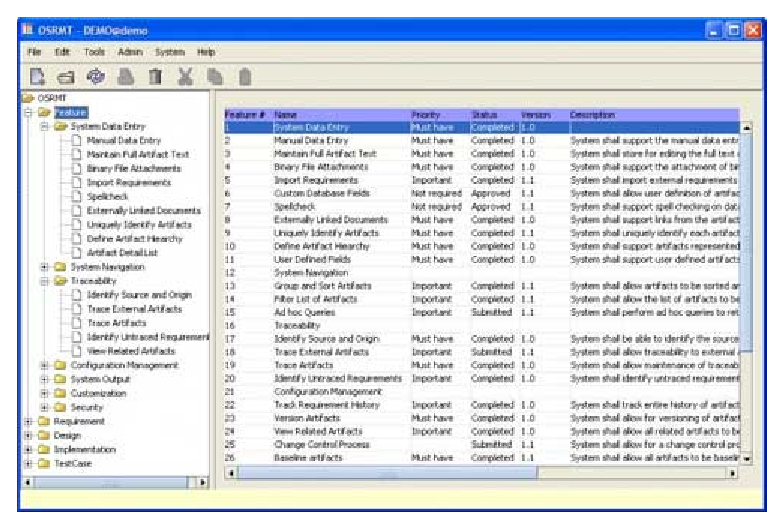
\includegraphics[keepaspectratio=true,scale=1.0]{figuras/ferramentasosrmt.eps}
\end{figure}

\subsection{Jira}

Jira é um software comercial pago desenvolvido pela empresa Australiana Atlassian. É uma ferramenta que permite o monitoramento de tarefas e acompanhamento de projetos, bem como para acompanhamento e reporte de defeitos em projetos de qualquer natureza. Esta ferramenta é baseada em Java EE que operam em vários Bancos de dados sendo estes: PostgreSQL, MySQL, Oracle e SQL Server para as versões 2005, 2008, 2012. O Jira é multiplataforma operando nos seguintes sistemas operacionais: Linux, Windows e Solaris \cite{jira2016}. 

O Jira possui alguns plugins para acompanhamento do progresso do projeto, com gráficos de pizza, gráficos de barra, filtro por versão, filtro por status dentre outros. Exemplos de alguns plugins para o Jira: BigTemplate, Workflow Tools and Functions (WTF) e em especial o plugin GreenHopper, que possibilita o usuário gerenciar projetos ágeis. 

A ferramenta oferece:
\begin{itemize}
    \item Possibilidade de registrar uma tarefa, classificar como bug, features ou itens de backlog;
    \item Incluir numa determinada versão;
    \item Indicar que a tarefa está sendo executada, que já foi executada ou que nem começou e quem é responsável por ela. 
    \item Controle de acesso e segurança customizado.
    \item Gestão de defeitos e incidentes: funcionalidades para criação, detalhamento e descrição de defeitos  ou incidentes e acompanhamento de resolução.
    \item Gestão de projetos: criação e delegação de projetos e tarefas, com fluxos de processos personalizados para o acompanhamento dos projetos.
    \item Integração com ambientes de desenvolvimento. \textbf{Exemplos:} Eclipse, Visual Studio, IntelliJ, Netbeans, entre outros.
    \item Importação de dados de outras ferramentas populares. \textbf{Exemplo:} Mantis.
\end{itemize} 

O Jira atende as principais tarefas de uma ferramenta de gerenciamento de requisitos de software. Esta ferramenta pode ser utilizado via web tendo suporte para os seguintes browsers: Microsoft Internet, Explorer, Mozilla Firefox, Google Chrome e Safari. Também pode ser instalado em um desktop ou notebook. A ferramenta requer um banco de dados e o Oracle JDK para funcionar \cite{jira2016}.
\begin{figure}[H]
    \centering
    \caption[Tela do software Jira]{Tela do software Jira. fonte: \url{https://wac-cdn.atlassian.com/software/jira/main/01/columns/00/content/0/localUpload/Backlog@2x.png.png?cdnVersion=k}}
    \label{jiraFerramenta}
    \includegraphics[keepaspectratio=true,scale=0.2]{figuras/jira.eps}
\end{figure}

\subsection{Innoslate}

Innoslate combina engenharia de software, analise de requisito ferramenta de colaboração. É um Model-Based Systems Engeneering software com gerenciamento, análise de requisitos e Departamento de defesa de arquitetura de Framework. Desenvolvido pela SPEC Innovations of Manassas

A ferramenta Oferece \cite{innoslate}:
\begin{itemize}
    \item Sugestão automática de numeração na criação de entidade, relações hierárquicas geradas automaticamente, filtrando classe de entidade e rótulos, exibição hierárquica com seções recolhíeis, edição entidade inline, indicadores de análise lacuna.
    \item O Rastreamento de requisitos diretamente para os elementos funcionais e físicas de um modelo de sistema, documentos de origem, planos de teste e outros requisitos, relacionamentos gerados automaticamente. A visualização da rastreabilidade através da Hierarquia gráfico ou um Rastreabilidade Aranha Diagram.
    \item Geração automática de um índice de qualidade para os requisitos. atributos de indicadores de qualidade \textit{built-in} melhorar cada requisito.
    \item Permite visualizar as versões antigas dos documentos criados podendo retorna-los, A toda mudança, atualização, modificação é gravada
    \item Permite deixar um comentário para membros de sua equipe, ou conversar com eles no chat ao vivo. Permite mantertoda a sua equipe de trabalho sobre a mesma versão dos requisitos do seu projeto com uma cópia centralizada do seu documento de requisitos em Innoslate.
    \item Criação de relatórios de verificação, validação e rastreabilidade.
\end{itemize}

Funciona em qualquer dispositivo (Mac, PC, iPad, Android) em qualquer navegador moderno (Google Chrome, Mozilla Firefox, Apple Safari, o Microsoft Internet Explorer 10+) com nenhuma instalação necessária \cite{innoslate}.
\begin{figure}[H]
    \centering
    \caption[Tela do software innoslate]{Tela do software innoslate. fonte: \url{https://www.innoslate.com/images/homepage-reqview.png}}
    \label{innoslateFerramenta}
    \includegraphics[keepaspectratio=true,scale=0.4]{figuras/innoslate.eps}
\end{figure}

\section{Escolha da ferramenta}
    
Para a escolha da ferramenta, foi elaborado critérios para avaliar as ferramentas selecionadas a base de pesquisas e indicações para garantir que a opção escolhida supre as necessidades do nosso contexto de negócio. A escolha dos critérios são baseadas nas atividades que desempenharemos no nosso processo, porém foi também levado em consideração os critérios \cite{hoffmann2004}:
A ferramenta escolhida

\subsection{Ferramenta escolhida}

Existem duas classificações importantes para a escolha de uma ferramenta de gerenciamento de requisitos, requisitos de desenvolvedores e requisitos de projetos administradores \cite{hoffmann2004}. Os requisitos de projetos administradores são para projetos de larga escala, e como o projeto em questão é um projeto de pequena e média escala, logo só serão tratados os requisitos de desenvolvedores.

\subsubsection{Critérios e metodologia de análise}

Para a escolha da ferramenta, foram escolhidos critérios baseados no Hoffmann (2004) e critérios elaborados pela equipe para se adequarem as necessidades da disciplina de engenharia de requisitos.
Para cada critério especificado, foi adotado um grau de prioridade para classificar a importância do critério para a escolha da ferramenta. Assim, é definido: 
\begin{description}
    \item '+++' - para alta prioridade; 
    \item '++' - média prioridade; 
    \item '+' - baixa prioridade;
\end{description}

A contagem para determinar a escolha da ferramenta, será definido pela soma de '+' que a ferramenta acumulou após a análise de todos os critérios estabelecidos.

\begin{itemize}
    \item \textbf{A abordagem adotada(+++):} a ferramenta deve ter suporte para a abordagem ágil, ou seja, dando suporte a Histórias de Usuário; Priorização de atividades; Backlog dentre outras atividades que o processo demanda relacionado a abordagem ágil;     
    \item \textbf{Matriz de Rastreabilidade(+++):} a ferramenta deve dar suporte a rastreabilidade dos requisitos às suas origens e os rastreamento durante todo o ciclo de vida do projeto. A ferramenta deve permitir a rastreabilidade através de links entre os requisitos, devendo ser possível seguir através desses links diretamente em ambos as direções \cite{hoffmann2004}.     
    \item \textbf{Acesso Web(+):} a ferramenta deve dar suporte a uma interface web para que não seja necessário instalar um aplicativo no computador para cada usuário que fará uso dela \cite{hoffmann2004}. Devendo também ter uma interface intuitiva e fácil de se manusear. O Jira oferece interface web intuitiva e fácil de utilizar.
    \item \textbf{Gestão de mudanças(++):} a ferramenta deve dar suporte para a gerenciamento de mudanças com base nas atividades desenvolvidas para lidar com essas modificações. Assim, com suporte ao gerenciamento de mudanças possibilita a redução de erros de forma significativa \cite{hoffmann2004}.
    \item \textbf{Comentários(+):} Deve permitir adicionar comentários aos requisitos, estes são para adicionar esclarecimentos necessários aos requisitos que não são simples de entender ou que usem referências externas \cite{hoffmann2004}.
    \item \textbf{Geração de relatórios(+):} a ferramenta deve dar suporte para a documentação de atividades realizadas e  prover a possibilidade de outros formatos de arquivos para programas externos a ferramenta.
    \item \textbf{Nível de documentação(+++):} o processo escolhido exige que seja permitido documentar os requisitos em quatro níveis: temas estratégicos, épicos, features e histórias de usuário.
\end{itemize}

\begin{table}[H]
    \centering
    \caption{Comparação entre ferramentas}
    \begin{tabular}{l|c|c|c}
        \hline
        Critérios & ScrumHalf &  Jira & Innoslate \\ [6pt]
        \hline
        Abordadem adotada & X & X & X\\
        \hline
        Matriz de rastreabilidade & X & X & X \\
        \hline
        Acesso Web & X & X & X \\
        \hline
        Gestão de mudanças & X & X & X\\
        \hline
        Comentários & X & X & X \\
        \hline
        Geração de relatórios & X & X & X \\
        \hline
        Resultados & 14 & 14 & 14 \\
    \end{tabular}
\end{table}

O Jira ofere suporte a abordagem ágil a partir de um plugin o GreenHooper ou o RMsis, ambos se adequam as nossas necessidades para a gerencia das atividades que serão realizadas. 
O Jira oferece suporte a matriz de rastreabilidade através de plugin um exemplo é o Traceability Matrix and Link Graph.
O Jira fornecer formas de assegurar que mudanças realizadas sejam controladas. Oferecendo a visibilidade de cada mudança efetuada no software, qual foi o motivo que gerou a mudança, quem executou dentre outras.
Jira fornece geração de documentos e exportação para WORD, PDF, XML e HTML \cite{jira2016}.

